%% LyX 2.1.4 created this file.  For more info, see http://www.lyx.org/.
%% Do not edit unless you really know what you are doing.
\documentclass[12pt,british]{article}
\usepackage[T1]{fontenc}
\usepackage[latin9]{inputenc}
\setlength{\parskip}{\smallskipamount}
\setlength{\parindent}{0pt}
\usepackage{babel}
\usepackage{float}
\usepackage{units}
\usepackage{amsmath}
\usepackage{graphicx}
\usepackage[unicode=true,pdfusetitle,
 bookmarks=true,bookmarksnumbered=false,bookmarksopen=false,
 breaklinks=false,pdfborder={0 0 1},backref=false,colorlinks=false]
 {hyperref}
\usepackage{breakurl}

\makeatletter
%%%%%%%%%%%%%%%%%%%%%%%%%%%%%% Textclass specific LaTeX commands.
\numberwithin{figure}{section}
\numberwithin{table}{section}
\numberwithin{equation}{section}

%%%%%%%%%%%%%%%%%%%%%%%%%%%%%% User specified LaTeX commands.
\usepackage {graphicx} 
\usepackage{color}
\usepackage{units}
\usepackage{textcomp}
%\usepackage{a4wide}
 \usepackage[a4paper, margin = 2cm, hmargin = 2cm, top = 1cm, includehead, includefoot, bindingoffse t= 1cm, twoside]{geometry} 
%\usepackage[charter]{mathdesign} 
%\usepackage{colortbl}
%\definecolor{lightgrey}{rgb}{0.59, 0.44, 0.09}
%\usepackage{url} 

%\setcounter{page}{-3}


%\usepackage{fancyhdr}
%\pagestyle{fancy}
%\setlength{\headheight}{15pt}
%\pagestyle{fancyplain}
%\renewcommand{\sectionmark}[1]{\markboth{#1}{}}
%\lhead{}

%\usepackage{wallpaper}

\makeatother

\begin{document}

\part*{The Muenster IceCube Display\protect \\
Software documentation}


\section{What you need}
\begin{itemize}
\item Hardware:

\begin{itemize}
\item $3\times$ Teensy 3.2 connected to computer via USB, power supply
and synchronized with each other
\item $1\times$ LED strip (at least) properly connected to one of the Teensys
and power supply
\item Power supply (both the Teensys and the LED strips need $\unit[5]{V}$)
\end{itemize}
\item Software

\begin{itemize}
\item IceTray software V17-03-00 \\
(\url{http://code.icecube.wisc.edu/svn/meta-projects/offline-software/releases/V17-03-00/})
\item Teensyduino (\url{https://www.pjrc.com/teensy/td_download.html}) and an Arduino version compatible with it (\url{https://www.arduino.cc/en/Main/Software})
\item Teensy Loader (\url{https://www.pjrc.com/teensy/loader.html})
\item Python package \texttt{pyusb} (get it with \texttt{pip} AND \texttt{pip3})
\item All the stuff that is in folders \texttt{muenster\_icecube\_display}
and \texttt{teensy32\_stuff}
\item A nice \texttt{.i3} file
\end{itemize}
\end{itemize}

\section{How to set this up}
\begin{itemize}
\item Test whether \texttt{pyusb} works correctly by running Python interactively
(should look something like the following):\\
\texttt{\$ python3}~\\
\texttt{Python 3.4.0 ...}~\\
\texttt{>\textcompwordmark{}>\textcompwordmark{}> import usb}~\\
\texttt{>\textcompwordmark{}>\textcompwordmark{}> usb.version\_info}~\\
\texttt{(1, 0, 0, 'b2)}
\item Add the following rules from the \texttt{teensy32\_stuff} folder so
you can run all scripts as normal user:\\
\texttt{\$ sudo cp 90-icecube.rules /etc/udev/rules.d/ }~\\
\texttt{\$ sudo groupadd leddisplay }~\\
\texttt{\$ usermod -a -G leddisplay {[}your username{]}}
\item Load the \texttt{.hex} file in the \texttt{teensy32\_stuff} folder
onto all three Teensys by means of the Teensy loader (explained on
the Teensy webpage)
\item Run the script \texttt{display\_info.py} from the \texttt{muenster\_icecube\_display}
folder to verify communication with the boards\\
\texttt{\$ python3 display\_info.py}
\item Now you have to load the display configuration (which strings are
located where in the model) onto the Teensys. You do this by means
of the \texttt{update\_eeprom.py} script and the configuration file
\texttt{display\_config\_muenster.json}. Should look something like
this:\\
\texttt{\$ sudo python3 update\_eeprom.py display\_config\_muenster.json
}~\\
\texttt{Found device }~\\
\texttt{Please select one of the available device configurations to
configure the device: }(enter \texttt{front}, \texttt{center} or \texttt{back}
here)\texttt{}~\\
\texttt{Selected configuration: Configuration uploaded. Please mark
the device to be able to match it with its serial number or configuration. Please
reboot the device for the new configuration to take effect.}
\item Verify wether writing new configuration worked by running \texttt{display\_info.py}
again; should get a slightly different output.
\end{itemize}

\subsection{Testing and debugging}
\begin{itemize}
\item The script \texttt{test\_draw.py} in the \texttt{muenster\_icecube\_display}
folder can be used for identifying your channels. The syntax is:\\
\texttt{\$ python3 test\_draw.py -m string -c 86 -d 1}~\\
The above command makes one string light up after the other (assuming
86 strings in total) for one second. Have a look at the script for
more options like rgb mode and offset.
\end{itemize}

\subsection{Controlling the display with steamshovel}
\begin{itemize}
\item Open steamshovel:\\
\texttt{\$ {[}directory of IceTray software{]}/build/ ./env-shell.sh
}~\\
\texttt{\$ steamshovel}
\item It is important at this point that the pyusb package is installed
via pip, since steamshovel runs on Python2 and not Python3
\item Click the button ``Add...'' on the right and select \texttt{LedDisplay()}
\item Select settings \texttt{I3Geometry} and e.g. \texttt{HLCPulses}
(see figure \ref{fig:steamshovel_screenshot_01})
\item When you run your .i3 file, the onboard LEDs on the Teensys should
flicker which means data is transmitted. The LED strips should light
up in synch with the steamshovel event.
\item HLCPulses if the cleanest service containing the pulses. They are triggered in time therefore only the event is shown. To produce this key (when it is not) and combine several files into only one, please use the script \texttt{/preparefiles/processing.py}.
\end{itemize}
\begin{figure}[H]
\noindent \begin{centering}
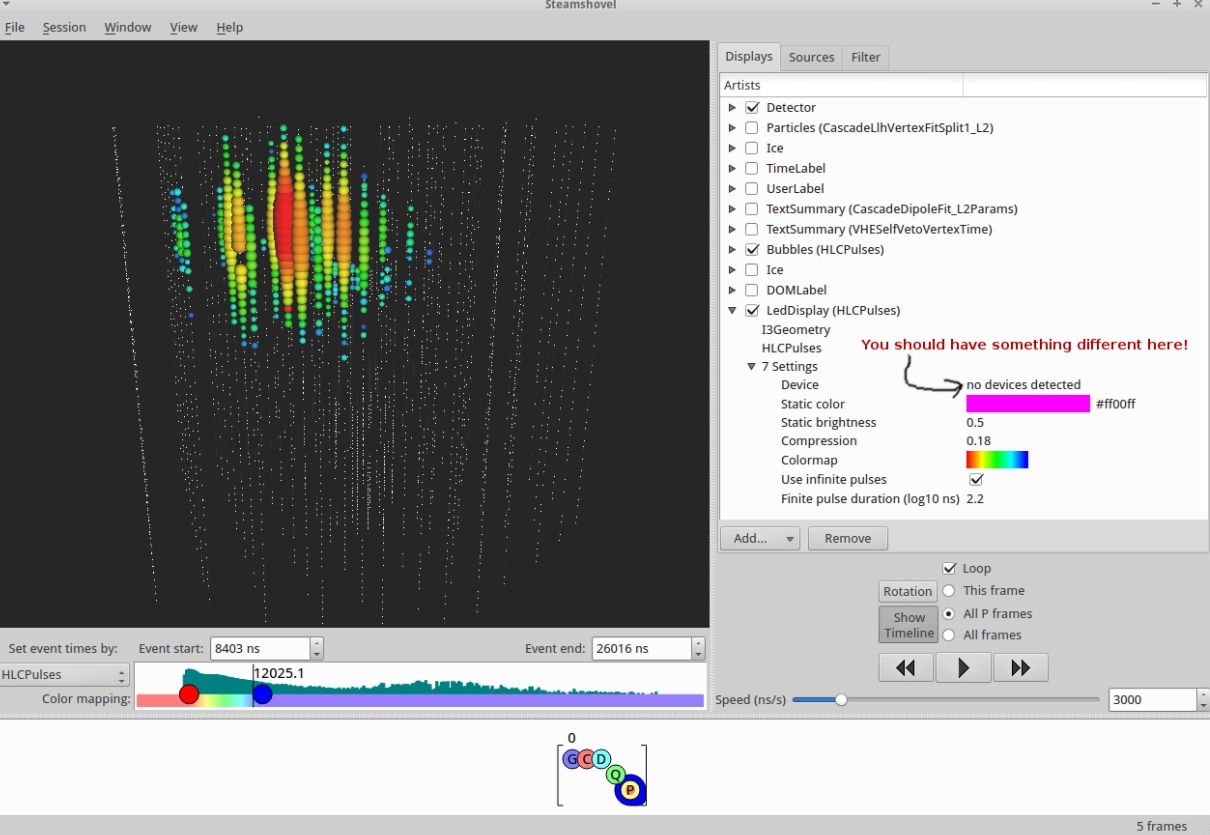
\includegraphics[width=1\textwidth]{steamshovel}\$ {[}directory of IceTray software{]}/build/ ./env-shell.sh

\par\end{centering}

\caption{\label{fig:steamshovel_screenshot_01}A steamshovel screenshot with
a possible configuration.}
\end{figure}

\section{Errors you might see when running it}
\begin{itemize}
\item After some loops, steamshovel breaks with an error as: \\
\texttt{\$ Could not write frame to controller \%s (USB errno 110 (maybe also 32))} \\
There is a overlap between the teensy and the computer (probably because your computer is too slow). To solve this, we have to increased the max. time that pyusb allows for comunication between the teensy and the computer. Open the following files with root rights: \\
\texttt{/usr/local/lib/python2.7/dist-packages/usb/legacy.py} \\
Go to the lines 144 and 156, you should be over the member functions \texttt{bulkWrite} and \texttt{bulkRead} inside class \texttt{DeviceHandle}. By default the timeout of both functions is 100 ms. Increase it to 1000 or 10000. This should solve the issue.
\item The led sometimes do blink/do something weird and you receive in the shell the following debug alert constantly: \\
\texttt{\$ Rendering too fast, cannot send more than 25FPS\footnote{The alert is only visible if Icetray was compiled with debug or higher verbosity level (by default it is)}} \\
Go to: \\
\texttt{\~IcetrayDirectory\~/src/steamshovel/python/artists/LedDisplay.py} \\
You have to modify the parameter \texttt{min\_delta} of the member function \texttt{transmitDisplayBuffer} inside the class \texttt{DisplayWorker} (line 501 in my version). Increase the render frequency by changing the default value of $1./25$ to $1./15$ or $1./10$. This might not totally solve the problem but it should \textbf{improve}. If the problem it is not totally solve, you will still have the debug alert in the shell (still with 25FPS if you didn't change the logger.debug on line 514). 
\item If you see more errors or are able to solve the last one, please write me to: \href{mailto:c\_loza01@uni-muenster.de}{c\_loza01@uni-muenster.de}
\end{itemize}
\end{document}
